%If you are presenting work which has been previously published, acknowledge this here.
% ***************************************************
% How to introduce a previously published chapter
% ***************************************************
%This is an example of how you might introduce a chapter that has been published previously. 
\cleartoevenpage
\pagestyle{empty}	
%Use this command (above) to suppress the header from the preceding chapter.

\noindent
The following publication has been incorporated as Chapter~\ref{Chap:label}.

\noindent
Manuscript in preparation.

\begin{table}[h]
	\centering
	\begin{tabular}{clr}
		\toprule
		Contributor & Statement of contribution & \% \\
		\midrule
		\textbf{Your Name}				& writing of text 					& 70\\
															& proof-reading							& 60 \\
															& theoretical derivations 	& 70\\
															& numerical calculations 		& 100\\
															& preparation of figures 		& 80 \\
															& initial concept						& 10 \\
		\midrule
		Co-author 1								& writing of text 					& 20\\
															& proof-reading							& 10 \\
															& supervision, guidance 		& 20\\
															& theoretical derivations 	& 10\\
															& preparation of figures 		& 20 \\
															& initial concept						& 10 \\
		\bottomrule
	\end{tabular}
\end{table}

Details TBA.

Code and materials are temporarily available at \href{https://cloud.rdm.uq.edu.au/index.php/s/CNfJKL68dKYPJYL}{https://cloud.rdm.uq.edu.au/index.php/s/CNfJKL68dKYPJYL} (password: "thesisreview").


% ***************************************************
% Example of an internal chapter
% ***************************************************
%This is an internal chapter of the thesis.
%If you have a long title, you can supply an abbreviated version to print in the Table of Contents using the optional argument to the \chapter command.
\chapter[Pama-Nyungan tree inference with phonotactics]{Pama-Nyungan tree inference with phonotactics}
\label{ch-pn-treebuilding}	%CREATE YOUR OWN LABEL.
\pagestyle{headings}

% ********* Enter your text below this line: ********

Historical linguistics in the 21st century has been shaped by a quantitative turn. Computational phylogenetic methods have been used to infer detailed trees for an expansive array of language families around the world. However, data innovation remains a priority for methodological development in this field. Most linguistic phylogenies are inferred from lexical cognate data alone, leaving untapped sources of evidence from other parts of language. To this end, prior study suggests that phonotactics, including frequency data from biphone sequences in wordlists, could be a novel source of phylogenetic signal. In this paper, we evaluate the capacity to capture the phylogenetic signal in phonotactics for the purposes of tree inference. We test whether the inclusion of phonotactic data, in conjunction with lexical cognate data, can strengthen phylogenetic tree inference. To do this, we take 2,236 binary phonotactic variables and 133 frequency-based phonotactic variables and combine them with existing lexical cognate data from 44 western Pama-Nyungan languages. We run a Bayesian Markov chain Monte Carlo (MCMC) approach on two competing phylogenetic models. In one, the tree is inferred jointly using the phonotactic data and lexical cognate data. In the other, two separate trees are inferred, one from phonotactic data and the other from cognate data alone. The models are compared by estimating marginal likelihoods and calculating a Bayes factor. We also compare the competing tree topologies and clade support values. We return indeterminate results. We find that compromises to the evolutionary model for frequency data, which were necessary to make the study computationally feasible, had the undesirable effect of preventing consistently stable MCMC convergence and reliable marginal likelihood estimation. We discuss the reasons for this and provide an outline of future research steps to evaluate whether these findings support a true negative result or merely reflect current limitations of the methodology.

\hypertarget{pn-tree-intro}{%
\section{Introduction}\label{pn-tree-intro}}

Methodological development in 21st century historical linguistics has been defined by the uptake and increasing ubiquity of quantitative methods, and in particular Bayesian phylogenetic methods for inferring language trees. Language trees, or phylogenies, have been inferred using these methods for language families in Australia \autocite[Pama-Nyungan:][]{bowern_computational_2012}, Asia \autocites[Aslian:][]{dunn_aslian_2011}[Dravidian:][]{kolipakam_bayesian_2018}, Africa \autocite[Bantu:][]{whiteley_revising_2019}, Oceania \autocite[Austronesian:][]{gray_language_2009}, the Americas \autocites[Chapacuran:][]{birchall_combined_2016}[Tupí-Guaraní:][]{michael_bayesian_2015}, and Europe \autocites[Indo-European:][]{gray_language-tree_2003}{chang_ancestry-constrained_2015} (to select just a few examples). The task of phylogenetic tree inference is intrinsically interesting to historical linguistics, which is centrally concerned with the genealogical classification of languages. But it is important beyond historical linguistics too. Access to highly detailed phylogenies is necessary for the continued uptake of phylogenetic comparative methods in typology (see \textbf{CHAP REF}), and phylogenies can be combined with other sources of evidence to investigate migration patterns and other questions of human history \autocites[e.g.][]{hunley_genetic_2008}{bouckaert_mapping_2012}{malaspinas_genomic_2016}{bouckaert_origin_2018}.

With a few exceptions \autocites[e.g.][]{dunn_structural_2005}{dunn_structural_2008}, most quantitative historical linguistic studies have inferred trees exclusively from lexical cognate data---binary characters coding whether each language contains a member of a set of related word forms in its lexicon. Phylogenetic tree inference from lexical data has been a tremendously successful enterprise. Results have tended to align with traditional historical linguistic classifications where previous classifications exist, while adding detail to the tree and generating new insights \autocite[for example, the identification of major divisions within the Pama-Nyungan family, linking smaller, previously-identified subgroups, based on early phylogenetic splits inferred by][]{bowern_computational_2012}. Nevertheless, lexical cognate data in isolation has some limitations. It is taxing to acquire, requiring high quality language documentation and considerable expertise on the part of the linguist to identify and distinguish genuine cognate words from chance resemblances. The historical signal in lexical data also contains noise from instances of lexical borrowing and undetected semantic shifts.

It is pertinent to consider whether other forms of linguistic data could supplement lexical data in linguistic phylogenetics---in this instance, phonotactic data that is relatively easy to extract automatically from wordlists. Interestingly, a similar parallel discussion is taking place in other phylogenetic sciences. In biology, \textcite{parins-fukuchi_use_2018} find that combining continuous-valued anatomical morphological characters with more traditional, categorically-valued genomic data can strengthen tree inference. In linguistics, \textcite{macklin-cordes_phylogenetic_2020} found phylogenetic signal in phonotactic data, suggesting that phonotactic data could be a profitable addition for inferring phylogenetic trees. That study, however, was limited to measuring phylogenetic signal by comparing the phonotactic data to an existing phylogenetic tree. This study goes further by putting phonotactics into the actual practice of phylogenetic tree inference and evaluating whether this produces stronger results than phylogenetic tree inference based on lexical cognate data alone.

In this study, we test the question of whether phylogenetic tree inference can be strengthened by inferring the phylogeny from a combination of lexical cognate data and phonotactic data, compared to more traditional phylogenetic tree inference using cognate data in isolation. To test this, we take a sample of 44 languages from the western branch of the Pama-Nyungan family, Australia. We take previously published lexical cognate data \autocite{bouckaert_origin_2018} and extract phonotactic data from wordlists from the Ausphon Lexicon database \autocite{round_ausphon-lexicon_2017}, a comparably segmented, phonemicised extension of the CHIRILA database \autocite{bowern_chirila_2016}. Two phonotactic datasets are extracted, following \textcite{macklin-cordes_phylogenetic_2020}. One is binary, coding the presence or absence of two-segment sequences (biphones) in a given language. The other is a sound class transition frequency dataset which records the frequency of a sequence of two natural sound classes, \(xy\), relative to all instances of the sound class \(x\) (i.e.~for all instances of sound class \(x\), how often is it followed by the sound class \(y\)?). We compare two phylogenetic models, one in which a single tree is inferred jointly from the cognate data and phonotactic data, and a second model containing two trees, one inferred from cognate data and the other inferred from phonotactic data separately. We compare the two using a standard, well-established method of model comparison in phylogenetics, which is to infer marginal likelihood estimates for each model and compare them by calculating the Bayes factor \autocites{kass_bayes_1995}{brown_importance_2007}. In this instance, our model comparison returns indeterminate results due to the failure of our phylogenetic models to converge consistently. The challenge we encounter is striking the right balance between a model that is rich and linguistically plausible, while simultaneously remaining within current computational constraints. This challenge, though difficult, is perhaps not entirely intractable, and we conclude the paper with a detailed discussion of what will be required in future research to evaluate phonotactics in phylogenetics more fully.

The paper proceeds with the methodology in Section \ref{pn-tree-methodology}, defining the research question, detailing the overarching structure of the experimental section that follows, and describing the construction of the language sample. There are four experimental sections that follow: A first preliminary test (Section \ref{prelim-1}), a second preliminary test (Section \ref{prelim-2}), the main test (Section \ref{main-test}) and a follow-up test (Section \ref{follow-up-test}). The discussion (Section \ref{pn-tree-discussion}) and conclusion (Section \ref{pn-tree-conclusion}) detail the study's limitations and future directions.

\hypertarget{pn-tree-methodology}{%
\section{Methodology}\label{pn-tree-methodology}}

\hypertarget{research-question}{%
\subsection{Research question}\label{research-question}}

This study tests the question of whether or not the addition of phonotactic data strengthens linguistic phylogenetic tree inference. To test this question, we infer a phylogeny of the western branch of Pama-Nyungan languages using lexical cognate data and phonotactic data and repeat this process twice---once in which the phylogeny is inferred jointly from cognate and phonotactic data and once in which separate trees are inferred from cognate data and phonotactic data. The strength of phylogenetic inference in each instance is evaluated by estimating and comparing log marginal likelihoods for each, and comparing the topologies and posterior clade support values of maximum clade credibility trees.

\hypertarget{experimental-design}{%
\subsection{Experimental design}\label{experimental-design}}

There are four test components in this study: two preliminary test components and two main test components. Preliminary testing consists of (1) evaluating the best-fitting evolutionary model for binary biphone data, and (2) tree inference using cognate data only, essentially aiming to replicate \textcite{bouckaert_origin_2018}. Model comparison is a regular step in linguistic phylogenetic studies, as typically a number of clock models, site models and other parameters are considered. In this study, the cognate data is sourced from a prior study \autocite{bouckaert_origin_2018} which already evaluated the best-fitting model for this particular set of data. Accordingly, we pass over this evaluative process and replicate as much as possible the best supported model and priors from \textcite{bouckaert_origin_2018}, which includes a covarion model with a relaxed clock and fixed rates across cognate classes. It is a different story, however, for the binary biphone data which has not been used previously for phylogenetic tree inference. The novelty of this data source necessitates a thorough evaluation of which evolutionary model can best be applied to it. This is the subject of the first preliminary test.

The second preliminary test involves inferring a phylogeny using only cognate data from \textcite{bouckaert_origin_2018}. This test functions as a sanity check to ensure that our phylogenetic model and software implementation, which approximates but does not exactly replicate \textcite{bouckaert_origin_2018}, produces suitably equivalent results.

These preliminary tests are followed by the main test evaluating the primary research question described above. We use the Bayesian Markov chain Monte Carlo (MCMC) method implemented in BEAST phylogenetic software to infer a phylogeny of western Pama-Nyungan using cognate data, binary biphone data and continuous phonotactic data consisting of sound class transition frequencies. In a second MCMC run, we include two tree models, one inferred with cognate data only and another with phonotactic data only (both binary and continuous). Marginal likelihoods are estimated using the stepping stone sampling method \autocite{baele_accurate_2013}. For each tree model, we produce a maximum clade credibility tree from the posterior sample of trees that BEAST produces and then compare the topologies and clade support values of these.

We conduct one follow-up test after this. To test our suspicion that the binary phonotactic data was contributing undue weight to likelihood calculations without contributing much phylogenetic information, we re-ran the experiment with this data partition removed. In this instance, the second BEAST run contains two tree models, one inferred with cognate data only and one inferred using cognate data and continuous phonotactic data together.

There are a couple of additional points on software and model design that hold throughout all four tests. Firstly, regarding the evolutionary model for frequency-based phonotactic characters, we take a standard, lightweight, Brownian motion model in which frequency values can wander up or down with equal probability through time. We are currently limited to this model by software constraints, but accept it as a reasonable starting point. Firstly, Brownian motion is a common starting point in comparable biological studies that jointly infer trees with continuous data. Secondly, it follows the model used in \textcite{macklin-cordes_phylogenetic_2020}. One difference between \textcite{macklin-cordes_phylogenetic_2020} and this study is that \textcite{macklin-cordes_phylogenetic_2020} use raw frequency values whereas we use logit-transformed frequency values.

We use a Bayesian computational approach to infer linguistic phylogenies using BEAST phylogenetic software (v1.10.5) \autocite{suchard_bayesian_2018}. This is similar to earlier work on the Pama-Nyungan phylogeny \autocites{bowern_computational_2012}{bouckaert_origin_2018} which used BEAST2 \autocite{bouckaert_beast_2019}. We selected BEAST over BEAST2 because it offers the ability to infer trees with continuous characters. Throughout, we generally follow \textcite{bouckaert_origin_2018} as closely as possible. We follow \textcite{bouckaert_origin_2018} in constraining the tree topology using clade priors for well-established and commonly accepted Pama-Nyungan subgroups, as established by \textcite{ogrady_languages_1966}, \textcite{muhlhausler_atlas_1996} and \textcite{koch_languages_2014} and subsequently recovered in computational phylogenetic analysis by \textcite{bowern_computational_2012}. Dating the Pama-Nyungan tree is a central focus of \textcite{bouckaert_origin_2018}, combining lexical cognate data with geographical data and archaeological calibration points to give a best-available estimate of the geographic and temporal point of origin of the family. Accordingly, we retain their calibration prior on the Wati subgroup, which places a 95\% probability of the subgroup's origin dating between 3,000-5,000 years, with most of the probability density skewing towards the younger end of that range (a gamma distribution of \(\alpha = 2\), \(\beta = 359\), with 3,000 year offset) based on a synthesis of archaeological evidence \autocite[see][p.~746]{bouckaert_origin_2018}. We place a prior on the root age of the Pama-Nyungan family centred on a mean of 5,791 years B.P., following the findings of \textcite{bouckaert_origin_2018}. 5,791 years is the mean root age of the posterior for their best supported hypothesis on Pama-Nyungan's origins. We model this as a normal distribution (SD = 730) approximating the 95\% range of posterior root age estimates. One aspect in which we differ from \textcite{bouckaert_origin_2018} is tip dates. \textcite{bouckaert_origin_2018} use a birth-death skyline tree model which allows for tip dates to differ and includes a parameter corresponding to the proportion of total taxa sampled at a given point in time. This is reasonable since they use language sources span over 200 years. In contrast, we assume all tips are contemporaneous. In our case, since we restrict attention to relatively modern sources, any extra precision to be gained from including tip dates is not worth the reduced tree model choice in BEAST and extra computational expense.

\hypertarget{language-sample}{%
\subsection{Language sample}\label{language-sample}}

The target language sample, in the first instance, is the 306 Pama-Nyungan language varieties represented in \textcite{bouckaert_origin_2018}. Of these, we restrict attention to languages meeting the following criteria. Firstly, the language must be represented in the Ausphon Lexicon database \autocite{round_ausphon-lexicon_2017} from which we source wordlist data. Secondly, the original wordlist data source must have been compiled by a trained linguist from primary fieldwork with living speakers or a combination of fieldwork and archival materials (no sources reconstituted only from archival materials). Thirdly, each wordlist must contain at least 250 lexical items. This leaves a subset of 112 Pama-Nyungan languages. In Preliminary Test 1, where computational demands are relatively minimal, this is the language sample we use. Due to computational constraints associated with large amounts of continuous data and large phylogenies, in the main test we restrict attention to the western branch of the Pama-Nyungan family identified in \textcite{bowern_computational_2012} and \textcite{bouckaert_origin_2018}. This gives a sample of 44 western Pama-Nyungan languages covering nine Pama-Nyungan subgroups. A list of the bibliographic details of original language sources is available in \textbf{APPENDIX REF}.

\hypertarget{prelim-1}{%
\section{Preliminary test 1: Evolutionary model for binary biphone data}\label{prelim-1}}

As the number of linguistic phylogenetic studies using lexical cognate data has grown, some consistent findings have emerged; for example, the covarion model now seems widely preferred \autocites[e.g.][]{bouckaert_origin_2018}{kolipakam_bayesian_2018}{savelyev_bayesian_2020}. However, this is to the best of our knowledge the first attempt at Bayesian phylogenetic tree inference with binary biphone characters (though see \textcite{jager_inferring_2016} for a similar approach using a distance-based tree inferencing method). Accordingly, we start by embarking on the process of model testing and selection for this novel data type. The aim is to identify a sensible model and set of priors that we can specify for the binary biphone data in subsequent testing.

For each model specification, we run two independent MCMC chains of 25,000,000 iterations, with parameters logged every 10,000 iterations. Log marginal likelihoods are estimated using BEAST's path sampling/stepping stone sampling procedure \autocite{baele_accurate_2013} consisting of 50 path steps of 500,000 iterations, with parameters logged every 10,000 iterations, conducted on each chain then combined to get an overall marginal likelihood estimate (MLE). We conducted autocorrelation and convergence checks using Tracer v1.7.1 software \autocite{rambaut_posterior_2018}. Note that the results here are a preliminary exploration of model parameters to determine the best parameter settings for the tree inference presented in Section \ref{pn-tree-combined} below. We do not anticipate that binary biphone characters will produce especially high quality or realistic language phylogenies on their own. The goal is to get a handle on how best to model the evolutionary dynamics of this dataset when used in combination with other sources of evidence.

We test a total of 16 models, consisting of each logically possible combination of site and clock model components. We describe each of these alternatives in turn below.

\hypertarget{binary-biphone-data}{%
\subsection{Binary biphone data}\label{binary-biphone-data}}

A language's phonotactic system consists of rules governing how phonemic segments may combine into larger syllables and words. To represent phonotactics, we extract data on the presence and frequencies of \emph{biphones}, two-segment sequences, from language wordlists. From each wordlist, we extract data on the presence and absence of \emph{biphones}, sequences of two segments (where each segment is either a phoneme or a word boundary). A biphone is marked `1' if it is present anywhere in a language's wordlist. If the biphone consists of two segments that are part of the language's phonemic inventory (and therefore the biphone could, in principle, occur in the language) but the biphone never occurs, it is marked `0' for absent. If one or both segments in the biphone are not part of the language's phonemic inventory, then it is marked as a gap `-' in the data. A total of 2236 binary biphone characters are extracted.

\hypertarget{site-and-clock-settings}{%
\subsection{Site and clock settings}\label{site-and-clock-settings}}

Site models describe how binary biphone characters evolve through time. The site model is defined by three parameters, giving eight possible combinations to test:

For this stage of evaluation, we fix the clock model to a strict clock (no variation in evolutionary rates between branches) and fix the tree model to a simple calibrated Yule tree model with a uniform birth rate prior (Yule tree models do not allow for extinction events). We then test all eight combinations of three site model parameters:

\begin{itemize}
\tightlist
\item
  A simple continuous time Markov chain (CTMC) model (which contains a single estimated parameter that specifies the frequencies with which biphones are gained and lost) versus a covarion model (which allows sites to switch between fast and slow states). The covarion model is the preferred model of lexical cognate evolution in \textcite{bouckaert_corrections_2012}, \textcite{bouckaert_origin_2018} and \textcite{kolipakam_bayesian_2018}, although \textcite[p.~219]{chang_ancestry-constrained_2015} find little difference between them and opt for the increased simplicity of the former model.
\item
  Empirical character state frequencies versus estimated character state frequencies.
\item
  Site homogeneity (fixed evolutionary rates across all character sites) versus heterogeneity (estimated using four gamma distributed categories, following \textcite{kolipakam_bayesian_2018}). For cognate data, \textcite{bouckaert_origin_2018} find a better fit with homogenous rates but \textcite{kolipakam_bayesian_2018} find a better fit with heterogenous ones.
\end{itemize}

We use Bayes factors \autocite{kass_bayes_1995} to determine the best supported site, clock and tree models. Bayes factors give an indication of the support for one model over another and are calculated by calculating the ratio of the log marginal likelihoods of each model. A Bayes factor of 5 to 20 is taken as substantial support, greater than 20 as strong support, and greater than 100 as decisive \autocite{kass_bayes_1995}. We table Bayes factors comparing each combination of model settings in Table \ref{tab:site-models}. The names of each model indicate site settings as follows: (S)imple CTMC versus (C)ovarion model, e(M)pirical versus e(S)timated character frequencies, (H)omogenous rates versus (G)amma-distributed heterogenous rates. So, for example, the model termed ``CMH'' consists of a covarion model with empirical frequencies and homogenous rates across all sites.

We test two clock models: A strict clock, in which a single evolutionary rate is fixed across all branches in the tree, and a lognormally-distributed, uncorrelated relaxed clock. This relaxed clock model generally has been found to outperform a strict clock when modelling lexical cognate evolution \autocites{bouckaert_origin_2018}{kolipakam_bayesian_2018}. Clock settings are denoted in Table \ref{tab:site-models} by `S' for strict and `R' for relaxed. So, for example, the model termed ``SSG-S'' is a simple site model with estimated character frequencies and gamma-distributed heterogenous rates, combined with a strict clock.

For the relaxed clock, we used an uncorrelated lognormal setting with a uniform prior {[}0,1{]} following \textcite{kolipakam_bayesian_2018}. \textcite{bouckaert_origin_2018} constrain the upper bound to 1.0E-4 to reduce burn-in time since, in practice, the mean clock value never approaches even that level. We chose the less informative upper bound given the uncertainty of working with a novel data type.

A third Bayesian phylogenetic model component is the tree model which defines the speciation process. Two main alternatives appear frequently in linguistic phylogenetic research. These are birth-death speciation models, which allow for extinction events, and Yule speciation models, which allow birth events only \autocites[as preferred in][]{bowern_computational_2012}{kolipakam_bayesian_2018}. \textcite{bouckaert_origin_2018} use a Birth-Death Skyline model which enables tips to be sampled at different dates, but fix the death rate to zero. This is reasonable since they use language sources span over 200 years. Throughout this study, we follow this precedent by using a birth-death model with the death rate set to zero. However, instead of including different tip ages, we assume all tips are contemporaneous and set their ages to 0, which is not strictly accurate since original wordlist sources do vary in age. In our case, since we restrict attention to relatively modern sources, any extra precision to be gained from including tip dates is not worth the reduced tree model choice in BEAST and extra computational expense. One additional parameter that we do include instead is an incomplete sampling parameter to account for the fact that our language sample is only a subset of the full 306 languages included in \textcite{bouckaert_origin_2018}. This incomplete sampling parameter is set to 0.366 in this preliminary test (\(\frac{112}{306}\)).

\hypertarget{results-prelim-1}{%
\subsection{Results}\label{results-prelim-1}}

Bayes factors of pairwise comparisons between candidate models are listed in Table \ref{tab:site-models}. These results can be broken down into some key findings as follows:

\begin{itemize}
\tightlist
\item
  The covarion model overwhelmingly outperforms the simple CTMC model in all instances.
\item
  Variable evolutionary rates are favoured over fixed rates. This will increase the computational demand of models in the main experiment later on, since it increases the number of parameters to be estimated. Models with heterogenous rates require 3--4 times as long as equivalent models with fixed rates.
\item
  There is decisive support for estimating character state frequencies rather than simply taking the observed frequencies when the covarion model is used, although the opposite is true with a CTMC model.
\item
  Using estimated frequencies seems more important than using heterogenous rates. A covarion model with estimated frequencies and disfavoured, homogenous evolutionary rates will score higher than a covarion model with heterogenous rates but disfavoured empirical frequencies.
\end{itemize}

All up, we determine the best site model to be a covarion model with estimated frequencies and rate heterogeneity.

With regards to the clock model, site models paired with a relaxed clock tend to do better than their direct equivalents paired with a strict clock, though covarion models with homogenous rates are exceptions. The best site model, denoted `CSG' (covarion, estimated frequencies, gamma heterogenous rates), scores decisively higher than all others regardless of which clock model is used. The `winning' model, which we proceed to apply to binary biphone data throughout the rest of this study, is the CSG model with a relaxed clock (`CSG-R').

\begin{sidewaystable}

\caption[Bayes factors for different site models]{\label{tab:site-models}Bayes factors for different site models. Each Bayes Factor represents the support for one model (vertical axis) against another (horizontal). A positive value indicates the first model (left) is supported, and conversely, a negative value indicates the second model (top) is supported. A value over 100 is considered decisive.}
\centering
\fontsize{8}{10}\selectfont
\begin{tabular}[t]{lrrrrrrrrrrrrrrrr}
\toprule
Site model & CMG-R & CMG-S & CMH-R & CMH-S & CSG-R & CSG-S & CSH-R & CSH-S & SMG-R & SMG-S & SMH-R & SMH-S & SSG-R & SSG-S & SSH-R & SSH-S\\
\midrule
CMG-R & -- & 20,274 & 44,531 & 20,746 & -33,840 & -16,924 & 42,417 & 22,034 & 59,797 & 59,966 & 61,049 & 61,250 & 59,793 & 59,932 & 61,036 & 61,246\\
CMG-S & -20,274 & -- & 24,257 & 472 & -54,114 & -37,198 & 22,143 & 1,760 & 39,523 & 39,692 & 40,775 & 40,976 & 39,519 & 39,658 & 40,762 & 40,972\\
CMH-R & -44,531 & -24,257 & -- & -23,785 & -78,371 & -61,455 & -2,114 & -22,497 & 15,266 & 15,435 & 16,518 & 16,719 & 15,262 & 15,401 & 16,505 & 16,715\\
CMH-S & -20,746 & -472 & 23,785 & -- & -54,586 & -37,670 & 21,671 & 1,288 & 39,051 & 39,220 & 40,303 & 40,504 & 39,047 & 39,186 & 40,290 & 40,500\\
\addlinespace
CSG-R & 33,840 & 54,114 & 78,371 & 54,586 & -- & 16,916 & 76,257 & 55,874 & 93,637 & 93,806 & 94,889 & 95,090 & 93,633 & 93,772 & 94,876 & 95,086\\
CSG-S & 16,924 & 37,198 & 61,455 & 37,670 & -16,916 & -- & 59,341 & 38,958 & 76,721 & 76,890 & 77,973 & 78,174 & 76,717 & 76,856 & 77,960 & 78,170\\
CSH-R & -42,417 & -22,143 & 2,114 & -21,671 & -76,257 & -59,341 & -- & -20,383 & 17,380 & 17,549 & 18,632 & 18,833 & 17,376 & 17,515 & 18,619 & 18,829\\
CSH-S & -22,034 & -1,760 & 22,497 & -1,288 & -55,874 & -38,958 & 20,383 & -- & 37,763 & 37,932 & 39,015 & 39,216 & 37,759 & 37,898 & 39,002 & 39,212\\
\addlinespace
SMG-R & -59,797 & -39,523 & -15,266 & -39,051 & -93,637 & -76,721 & -17,380 & -37,763 & -- & 169 & 1,252 & 1,453 & -4 & 135 & 1,239 & 1,449\\
SMG-S & -59,966 & -39,692 & -15,435 & -39,220 & -93,806 & -76,890 & -17,549 & -37,932 & -169 & -- & 1,083 & 1,284 & -173 & -34 & 1,070 & 1,280\\
SMH-R & -61,049 & -40,775 & -16,518 & -40,303 & -94,889 & -77,973 & -18,632 & -39,015 & -1,252 & -1,083 & -- & 201 & -1,256 & -1,117 & -13 & 197\\
SMH-S & -61,250 & -40,976 & -16,719 & -40,504 & -95,090 & -78,174 & -18,833 & -39,216 & -1,453 & -1,284 & -201 & -- & -1,457 & -1,318 & -214 & -4\\
\addlinespace
SSG-R & -59,793 & -39,519 & -15,262 & -39,047 & -93,633 & -76,717 & -17,376 & -37,759 & 4 & 173 & 1,256 & 1,457 & -- & 139 & 1,243 & 1,453\\
SSG-S & -59,932 & -39,658 & -15,401 & -39,186 & -93,772 & -76,856 & -17,515 & -37,898 & -135 & 34 & 1,117 & 1,318 & -139 & -- & 1,104 & 1,314\\
SSH-R & -61,036 & -40,762 & -16,505 & -40,290 & -94,876 & -77,960 & -18,619 & -39,002 & -1,239 & -1,070 & 13 & 214 & -1,243 & -1,104 & -- & 210\\
SSH-S & -61,246 & -40,972 & -16,715 & -40,500 & -95,086 & -78,170 & -18,829 & -39,212 & -1,449 & -1,280 & -197 & 4 & -1,453 & -1,314 & -210 & --\\
\bottomrule
\end{tabular}
\end{sidewaystable}

One limitation to note is that we have not considered the stochastic Dollo model, which has been implemented with some success for cognate data in linguistics \autocite{bowern_computational_2012} (although the covarion model was subsequently found to be better in \textcite{bouckaert_origin_2018}). Stochastic Dollo only allows characters to spring into existence once and any losses are permanent. Such a model is perhaps a bit more realistic for cognates, since the state space of possible words is practically infinite (i.e.~the chance of different people inventing the same word for the same thing independently is low, although of course it does happen sometimes)\footnote{As an aside, the stochastic Dollo model is not particularly realistic for cognates either since it does not allow for borrowing, which manifests as two independent origin points when plotted on a phylogenetic tree. The presence of borrowing likely explains why the covarion model tends to work better than stochastic Dollo in linguistic phylogenetic studies. As an aside, an ideal phylogeographic model of cognate evolution would allow for independent points of origin at two rates of likelihood: a very low rate of likelihood of the cognate originating independently anywhere throughout the tree (capturing the likelihood of undetected chance resemblances coded as cognates), and a relatively high likelihood of a cognate independently originating in languages that are geographically adjacent to a cognate where the cognate is already present (to capture effectively borrowing events rather than genuine instances of convergent evolution). However, this would almost certainly be computationally expensive.}. By contrast, there are only so many possible biphone combinations, many unrelated/distantly related languages share biphones (consider, for example, shared biphones between English and Pama-Nyungan languages) and it seems unreasonable to assume a single common point of origin for all of them. For this reason we disregarded the Dollo model for this study.

\hypertarget{prelim-2}{%
\section{Preliminary test 2: Tree inference using cognate data only}\label{prelim-2}}

This second preliminary test aims to replicate the results of \textcite{bouckaert_origin_2018} using the same cognate data and approximately the same evolutionary model. The goal is to ensure that our particular software implementation and slight differences in implementation of the evolutionary model do not unduly impact the results, which we then use as a baseline for comparison in the main test below.

Differences between the implementation of this test and \textcite{bouckaert_origin_2018} are as follows. Firstly, the language sample is greatly reduced. Owing to the computational demands of inferring a large phylogeny with a large quantity of continuous-valued data, the language sample for the main test is reduced to 44 western Pama-Nyungan languages and so this is the language sample we use here. Secondly, we include an incomplete sampling parameter of 0.537, to account for the fact that our language sample covers 44 of the 82 languages in the western branch of the \textcite{bouckaert_origin_2018} phylogeny. Another difference is that, as described above, we do not include divergent tip ages in our model, although the 44 languages we use are sourced from modern sources anyway. Finally, we run the model in BEAST software (v1.10.5) \autocite{suchard_bayesian_2018} rather than BEAST2 \autocite{bouckaert_beast_2019}. We selected BEAST over BEAST2 because it offers the ability to infer trees with continuous characters (necessary for the main test below).

We follow \textcite{bouckaert_origin_2018} in constraining the tree topology using clade priors for well-established and commonly accepted Pama-Nyungan subgroups, as established by \textcite{ogrady_languages_1966}, \textcite{muhlhausler_atlas_1996}, \textcite{koch_languages_2014} and \textcite{bowern_computational_2012}. There are 9 of these subgroups represented in our language sample: Kanyara-Mantharta, Kartu, Marrngu, Ngayarta, Ngumpin-Yapa, South-West, Thura-Yura, Wati, and Arandic (though Arandic is represented by a solitary language in this study, Western Arrernte, so a clade constraint on this subgroup would have no effect). Dating the Pama-Nyungan tree is a central focus of \textcite{bouckaert_origin_2018}, combining lexical cognate data with geographical data and archaeological calibration points to give a best-available estimate of the geographic and temporal point of origin of the family. Accordingly, we retain their calibration prior on the Wati subgroup, which places a 95\% probability of the subgroup's origin dating between 3,000-5,000 years, with most of the probability density skewing towards the younger end of that range (a gamma distribution of \(\alpha = 2\), \(\beta = 359\), with 3,000 year offset) based on a synthesis of archaeological evidence \autocite[see][p.~746]{bouckaert_origin_2018}. We place a flat, uniform prior on the root age of the western Pama-Nyungan phylogeny of 3,000--7,000 years. This covers the time period from the youngest possible age of the Wati subgroup to the oldest end of the age range of the Pama-Nyungan family as a whole, under the best supported hypothesis of the origin of the Pama-Nyungan family in \textcite{bouckaert_origin_2018} (the mean root age in that study is 5,791 years). If the Wati age prior and best supported Pama-Nyungan root age in \textcite{bouckaert_origin_2018} are accepted, it follows that this is the logically maximal age range in which the origin of the western Pama-Nyungan branch must lie.

\hypertarget{results-prelim-2}{%
\subsection{Results}\label{results-prelim-2}}

We run four independent MCMC chains of 100 million iterations each and discard the initial 10\% burn-in. Logs were inspected and combined in Tracer (v1.7.1) to confirm that each run converged properly in the same probability space and that ESS values for all parameters were sufficiently high (\textgreater{}200). Chains 1--2 converge nicely in the same space, with all ESS values over 800. Chain 3 got stuck in a local optimum in the state space and chain 4 failed to converge, so these were discarded. Chains 1--2 were combined with 10\% burn-in on each, giving a 180-million-state tree sample and combined ESS figures all greater than 1,900. A maximum clade credibility tree was produced using TreeAnnotator (v1.10.4). This is displayed in Figure \ref{fig:cogs-vs-bba2018} next to the same subset of languages from the maximum clade credibility tree in \textcite{bouckaert_origin_2018}. We recover largely the same topology with some minor differences. These discrepancies seem approximately equivalent to the level of discrepancies between the \textcite{bouckaert_origin_2018} phylogeny and phylogenies from \textcite{bowern_computational_2012} and \textcite{macklin-cordes_phylogenetic_2020}.

Western Arrernte, the sole representative of the Arandic subgroup, shifts places among deeper nodes in the tree. The internal structure of the Ngumpin-Yapa subgroup also differs, which is interesting since the internal structure of Ngumpin-Yapa also shifts between \textcite{bowern_computational_2012} and \textcite{bouckaert_origin_2018}. In other words, in this instance divergences exist in a subgroup of the tree where there was already uncertainty between different analyses. Overall, notwithstanding these discrepancies, we are content that our model and method is working as it should with cognate data.

\begin{figure}
\centering
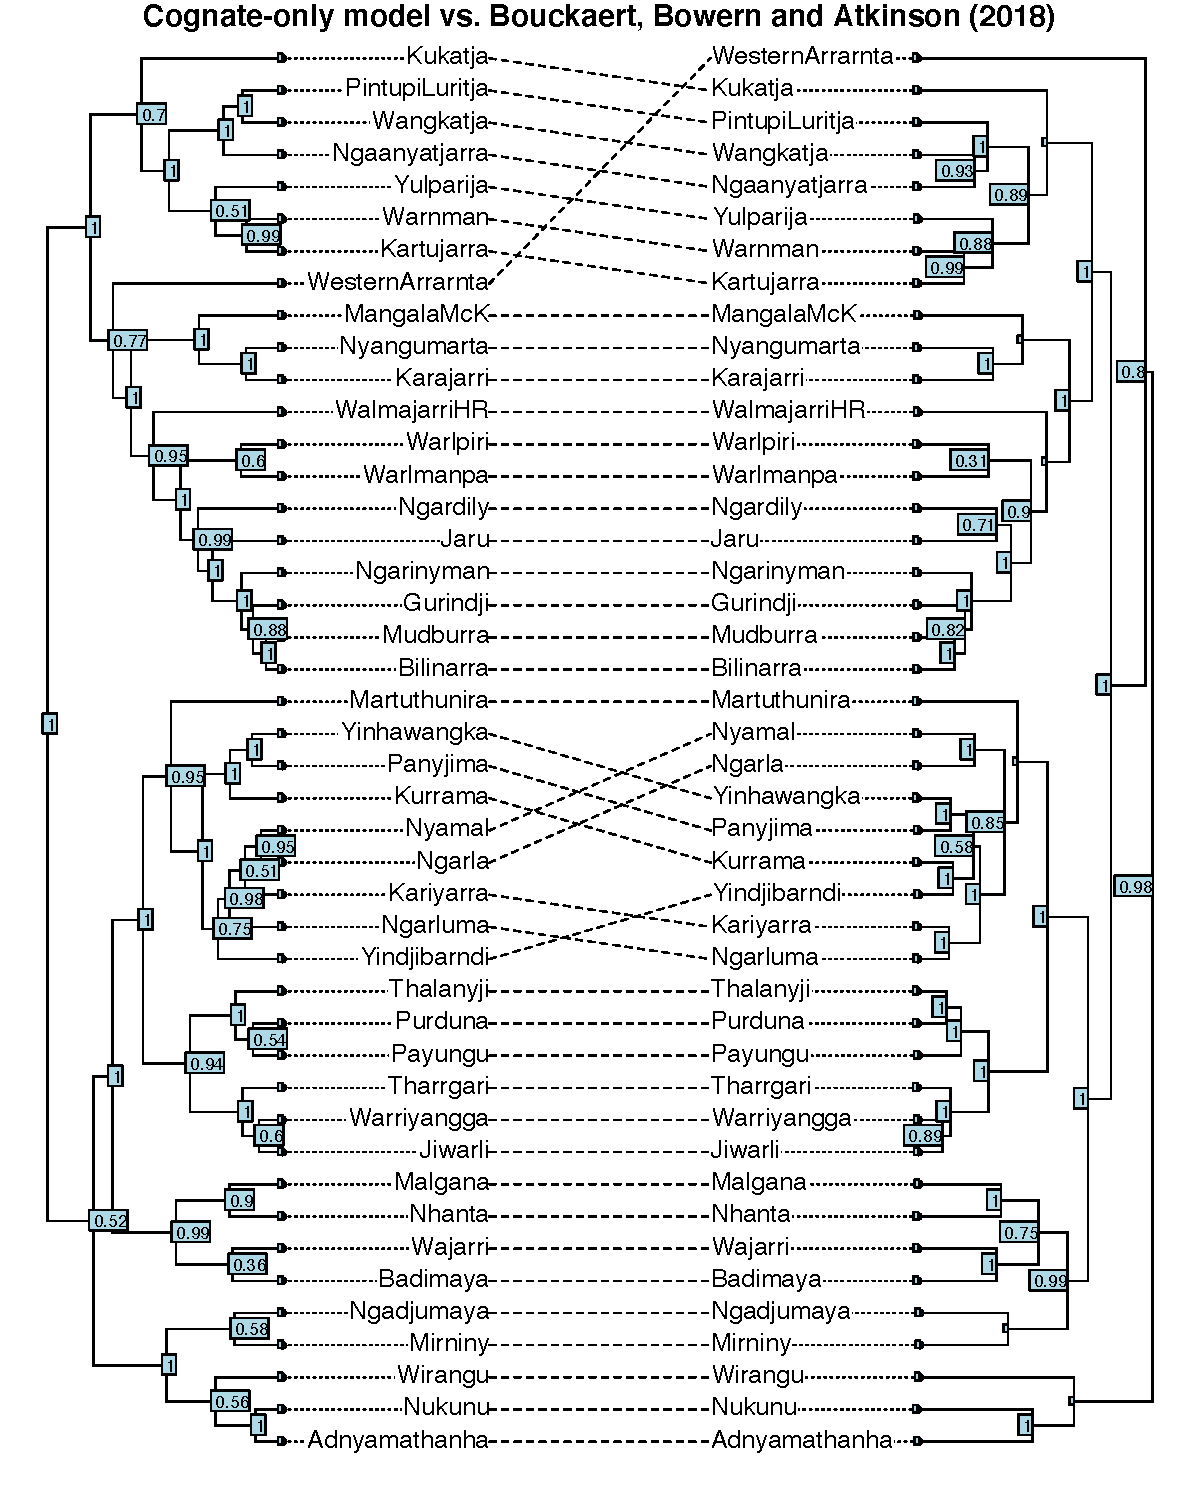
\includegraphics{06-tree-inference/fig/cogs_vs_bba2018.pdf}
\caption[Maximum clade credibility trees of our cognates-only model and the Bouckaert, Bowern \& Atkinson (2018) phylogeny]{\label{fig:cogs-vs-bba2018}The maximum clade credibility trees of our cognates-only model (left) and the Bouckaert, Bowern \& Atkinson (2018) phylogeny (right). Our model aims to replicate the BBA phylogeny as close as possible, although the language sample is restricted and there are some small model and software differences. Overall, the trees are mostly congruent, which gives reassurance that our baseline model is reliable.}
\end{figure}

\hypertarget{main-test}{%
\section{Main test: Tree inference with phonotactic data}\label{main-test}}

\hypertarget{data}{%
\subsection{Data}\label{data}}

There are three main sources of data for this experiment. One is cognate data from \textcite{bouckaert_origin_2018}, to which we apply an evolutionary model following \textcite{bouckaert_origin_2018}, as evaluated in Preliminary Test 2 (Section \ref{prelim-2}). There are two sets of phonotactic data, one binary and one continuous. Binary biphone data, which codes the presence or absence of biphones---sequences of two phonemes---in each language, is included with the best supported evolutionary model evaluated in Preliminary Test 1 (Section \ref{prelim-1}). Finally, we use a dataset of continuous phonotactic characters coding frequencies of transitions between natural sound classes. The data extraction process is detailed further as follows. Each consonant phoneme appearing in our wordlist data is binned into two natural classes, one for place of articulation and one for manner of articulation. Place classes are labial, dental, alveolar, retroflex, palatal and velar. Manner classes are obstruent, nasal, vibrant, lateral, glide, and rhotic glide. For the purposes of this experiment, we group all vowels into a single `vowel' class and also include word boundaries. The choice of place and manner natural classes is based on well-established principles of organisation among segments in Australian languages \autocites{dixon_languages_1980}{hamilton_phonetic_1996}{baker_word_2014}{round_segment_2021}{round_phonotactics_2021}. From each wordlist, we extract the frequency of a sound class \(x\) followed by a sound class \(y\), relativised over all instances of sound class \(x\). For use in BEAST, we logit-transform all the data to move from a 0--1 frequency interval to the real line. To include 0 and 1 frequency values in the logit-transformation, we follow a standard procedure of converting 0 values to \(\frac{min}{2}\), i.e.~half the smallest non-zero value, and converting 1 values to \(0.5 (1 + max)\), i.e.~half way between 1 and the maximum value less than 1. The evolutionary model applied to sound class transition frequency data in BEAST is a simple Brownian motion model which allows character values to wander up or down with equal possibility. We initially considered applying a single multivariate Brownian motion model to all continuous traits, however, the computational memory and time required by a multivariate Brownian motion model scales exponentially as the number of characters is increased. Instead, we fit a Brownian motion model to each character individually. This greatly increases the number of parameters in the overall model and potentially makes it less realistic, but it keeps the project computationally feasible. We return to this topic further in the discussion.

The choice of phonotactic data warrants brief further comment. We select sound class transition frequency data for a few reasons. One is that it partially, though not entirely, accounts for a lack of independence between biphone characters. This is because phonological rules, phonotactic restrictions and historical sound changes typically affect natural classes of phonemes rather than individual phonemes. This is not a perfect solution---sound classes themselves are independent from one another to varying degrees. A second reason is that \textcite{macklin-cordes_phylogenetic_2020} find a stronger degree of phylogenetic signal in sound class transition frequency data compared to transition frequencies between individual phonemes. A third reason is computational. A dataset of continuous characters equivalent in size to the binary biphone dataset would increase the computational time required to run BEAST by orders of magnitude, rendering the study impractical.

The decision to focus on frequency data in particular also warrants further explication. Notwithstanding the computational limitations we encounter, frequency data offers a number of possible advantages for phylogenetic inference. One is that it allows us to capture a finer grained level of information than binary data would allow. Binary data is more similar to the kind of phonotactic information one might find in a published language grammar, where a description of phonotactics that one would typically encounter involves a series of statements on the (binary) permissibility or otherwise of certain combinations of segments or natural classes of segments. This information does not, however, account for quantitative differences between common, high frequency sequences versus disfavoured sequences that rarely arise in a language's lexicon. There is considerable evidence to suggest that speakers are psychologically attuned to these kinds of phonological frequencies \autocites{coleman_stochastic_1997}{zuraw_patterned_2000}{ernestus_predicting_2003}{albright_rules_2003}{eddington_spanish_2004}{hayes_stochastic_2006}{gordon_phonological_2016}. The second reason is that the relatively rapid, semi-automated extraction of transition frequencies from wordlists captures structural variation between languages at a scale and degree of precision that would be difficult to attain from manual data coding methods (as preferred for the coding of lexical cognate data and grammatical data used in previous linguistic phylogenetic work). \textcite{macklin-cordes_phylogenetic_2020} show that this transition frequency dataset contains stronger phylogenetic signal than its binary equivalent. Increasing variation by shifting from categorical-valued characters to continuous characters has also been noted as advantageous for phylogenetics in biology, in the context of anatomical morphological data \autocites{parins-fukuchi_use_2018}{wright_systematists_2019}. An additional advantage is that our method avoids observer bias. We don't have to rely on an expert picking and choosing which parts of a grammatical or lexical system are interesting and worth coding. This has been noted as an advantage of large-scale extraction of continuous morphological characters in biology too \autocite{wright_systematists_2019}. Lastly, since we automatically extract frequencies for all possible biphones, we do not need to correct for acquisition bias or ascertainment bias \autocite{leache_short_2015}.

There is one limitation of the frequency data, which is that the Brownian motion model requires values above 0 and below 1. As described above, 0 values and 1 values are transformed to values very slightly above 0 and very slightly below 1 prior to logit-transformation. The inclusion of binary data in this study as well as frequency data is partly an effort to retain 0 and 1 values, which can be linguistically meaningful. One final limitation is that, throughout, our phonotactic data concerns linear sequences of exactly two segments. This is phonotactics in the simplest sense, and does not directly capture phonotactic restrictions that depend on sequences beyond two segments, syllable structure or morpheme boundaries. Nevertheless, \textcite{macklin-cordes_phylogenetic_2020} confirm that this simple level of phonotactic data is sufficient to detect strong phylogenetic signal.

As mentioned in Section \ref{prelim-2}, we reduce the language sample to 44 western Pama-Nyungan languages. This was necessary to keep the computational demands of the experiment reasonable. We selected the western branch of Pama-Nyungan due to it being relatively well-attested in modern sources compared to those in, for example, the south-east of Australia where language documentation is more often reliant on archival sources due to the disproportionate impact of colonialism in this part of the continent.

We run BEAST on two phylogenetic models: a `linked' model, which contains a single tree likelihood term calculated using all cognate and phonotactic data, and a `separate' model, which contains two tree likelihood terms, one calculated using cognate data only and the other using phonotactic data only (both binary and continuous). We run ten independent MCMC chains of 100 million iterations on each model, inspect and combine the results, estimate marginal likelihoods for each of the `linked' and `separate' models and generate three maximum clade credibility trees (one for the `linked' model, and one each for the cognate-only and phonotactics-only elements of the `separate' model).

\hypertarget{main-results}{%
\subsection{Results}\label{main-results}}

One first observation is that the MCMC process in BEAST tends to get stuck in local optima within the probability space and occasionally fails to converge. When this became clear, we increased the number of independent chains from an initial four to ten. Inspecting the joint probability traces for each of the linked model's ten runs, we find one clearly preferred area of the state space (Figure \ref{fig:linked-all-trace}). We remove two clear outliers stuck in local optima above and below the others. Two additional runs (visible in Figure \ref{fig:linked-all-trace} as two overlapping, slightly bimodal distributions, just to the left of the bulk of other chains) are removed since, although they overlap considerably with the others, they too seem to represent a distinct local optimum in the state space (one of these also failed to reach stable convergence). Three more chains failed to reach stable convergence after a reasonable (10--20\%) burn-in period and had to be removed. This leaves three stable chains with suitably high ESS values and consistent areas of convergence (the three tallest, central peaks in Figure \ref{fig:linked-all-trace}). The combined ESS for joint probability is 196. Over 200 would be preferable but we accept this as marginally acceptable. After discarding 10\% burn-in, we are left with a combined 270-million-state analysis.

BEAST computes two marginal likelihood estimates, one via the path sampling method \autocite{baele_improving_2012} and one via the stepping stone sampling method \autocite{baele_accurate_2013}. In normal operation these two estimates should be roughly equivalent. In this instance, the log marginal likelihood estimates for the combined analysis are 598,885 (estimated via path sampling) and 988,231 (estimated via stepping stone sampling). Currently, it is unclear whether or not these log MLE figures are meaningful. Log MLEs for each individual chain vary between 459,380 and 672,466 which is considerably more variation than we would expect, given that a difference of 20 is generally considered significant. Given that all chains represent the same data and model and converge in approximately the same space, we would expect their log MLEs to be around the same and certainly not as divergent as this. We discuss this further below.

\begin{figure}
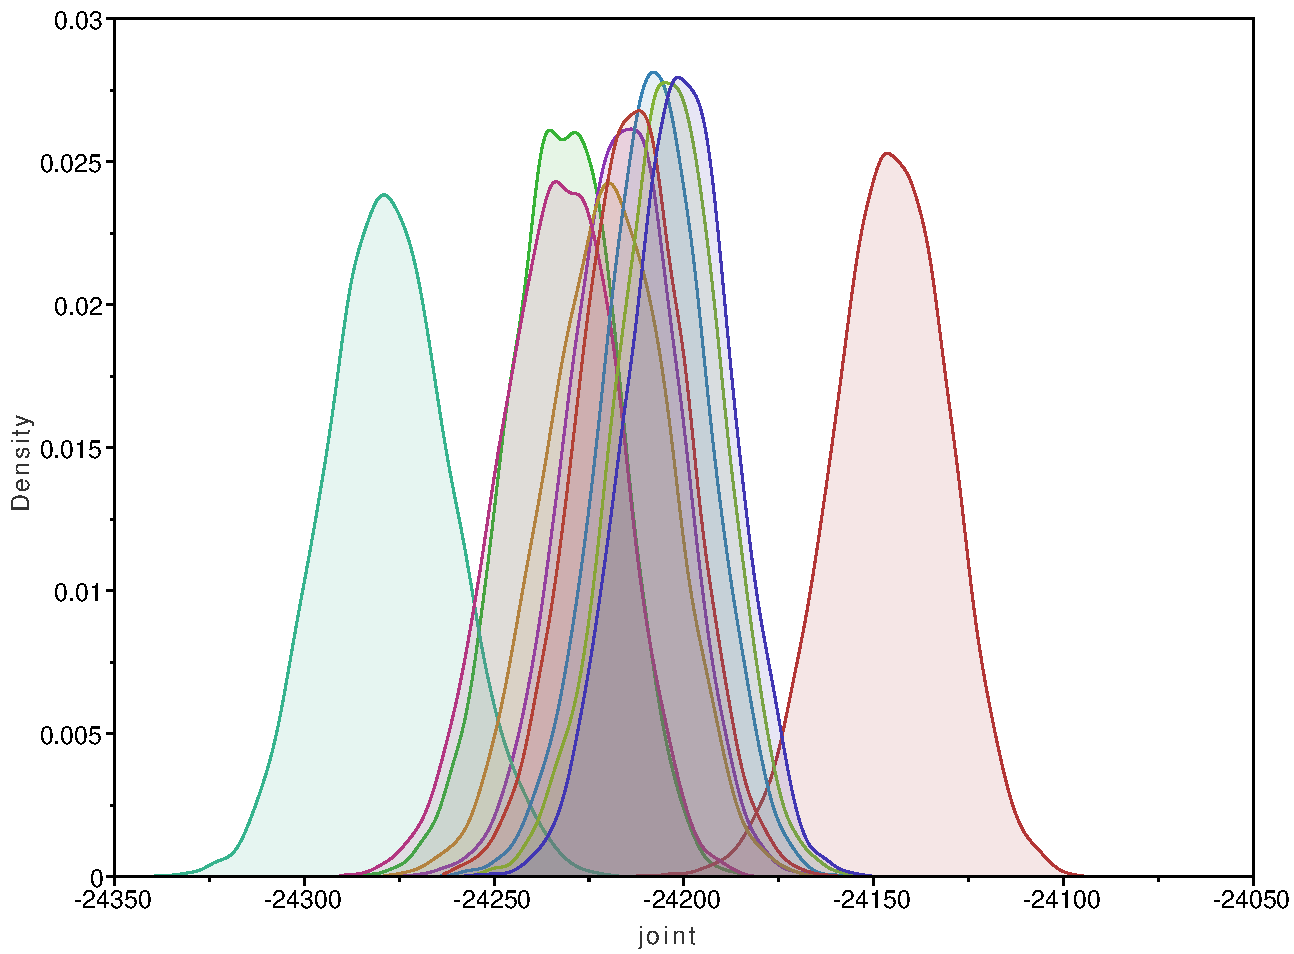
\includegraphics[width=0.5\linewidth]{06-tree-inference/fig/joint_trace_dens_ch1-10} 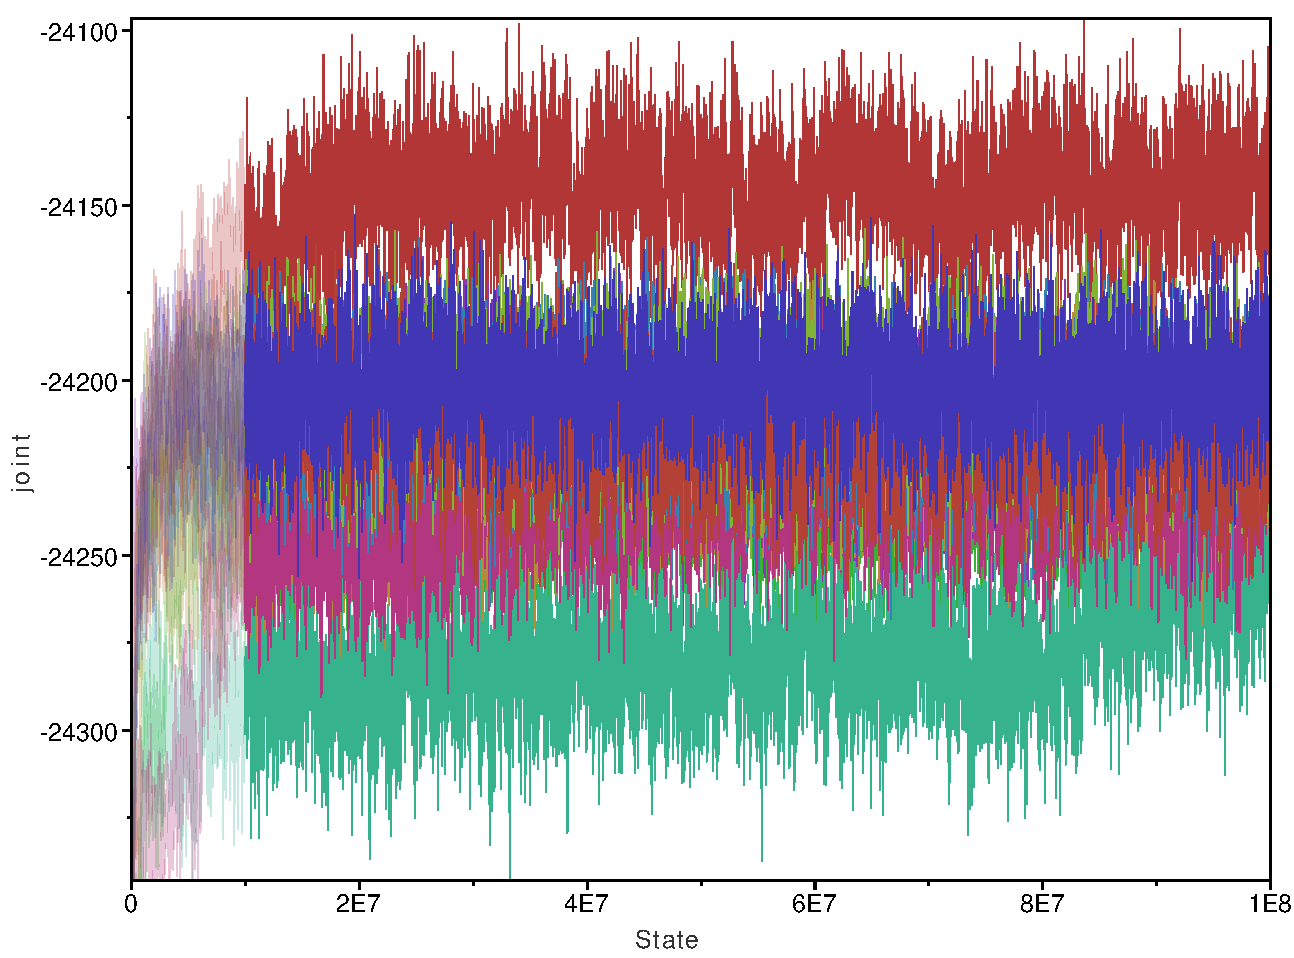
\includegraphics[width=0.5\linewidth]{06-tree-inference/fig/joint_trace_ch1-10} \caption[MCMC joint probability traces for the linked model]{MCMC joint probability traces for the linked model. Although a preferred general area of the probability space emerges, this area has wide bounds. There are two clear outliers and there is a considerable degree of inconsistency between chains.}\label{fig:linked-all-trace}
\end{figure}

The separate model, in which two trees are sampled at each step, one inferred using only cognate data and one inferred using only phonotactic data, fails to reach stable convergence and gives unacceptably low ESS figures in most instances. With a burn-in of 15\%, as per the linked model above, only 3 chains give a stable posterior sample with satisfactory ESS values. A fourth stabilises after a 20\% burn-in, and three others eventually stabilise in similar areas of the probability space to the others, but only after burn-in values of 50\%, 60\% and 70\%. We apply a consistent 20\% burn-in to the four most stable chains and discard the rest. Two of these converge in the same area while the other two converge in spaces of slightly lower joint likelihood. On this evidence, it is not entirely clear which is the most correct posterior distribution. We accept the two higher likelihood chains space as it makes the study's null hypothesis deliberately harder to reject (the null hypothesis that the joint model is no better than the separate model is harder to reject if we raise the bar set by the separate model). This gives a posterior sample of 160 million states and a marginally satisfactory ESS of 100 or greater for all parameters. Maximum clade credibility trees for each of the two tree elements---one inferred only with cognate data and the other inferred only with phonotactic data---are depicted in Figure \ref{fig:separate-cogs-vs-phonotactics-all}.

\begin{figure}
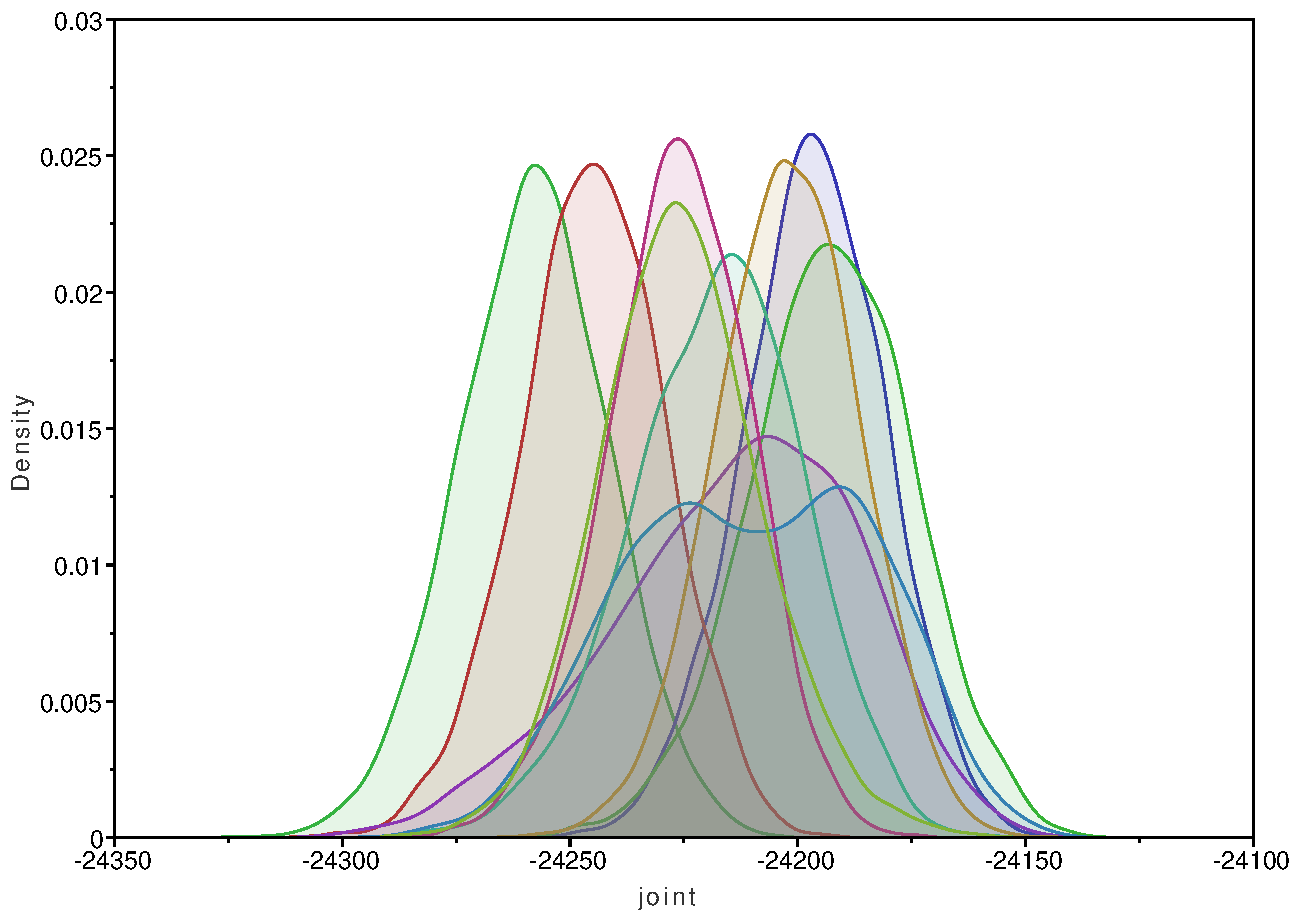
\includegraphics[width=0.5\linewidth]{06-tree-inference/fig/sep_trace_ch1-10} 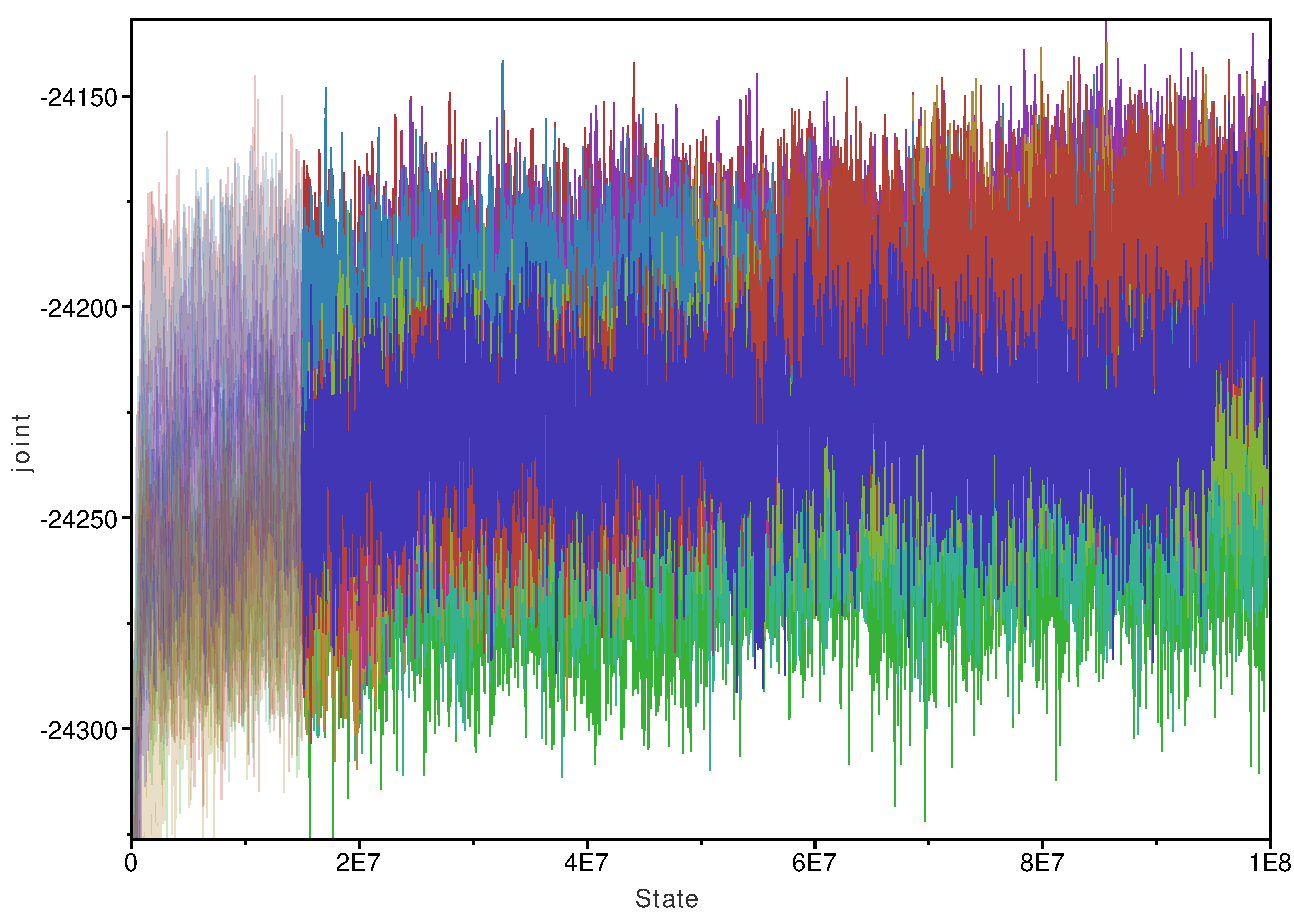
\includegraphics[width=0.5\linewidth]{06-tree-inference/fig/sep_trace_dens_ch1-10} \caption[MCMC joint probability traces for the separate model]{MCMC joint probability traces for the separate model. The lack of consistent (as seen on the left) and stable convergence (as seen on the right) is readily apparent.}\label{fig:separate-all-trace}
\end{figure}

The log MLEs for the separate model are 348,287 (estimated via path sampling) and 568,402 (estimated via stepping stone sampling). These MLEs can be compared with MLEs for the linked model in Table \ref{tab:linked-vs-separate-mles}. The linked and separate models can be compared using Bayes factors, following Equation \eqref{eq:bf}.

\begin{equation}
BF = log(MLE_{linked}) - log(MLE_{separate})
\label{eq:bf}
\end{equation}

The sign of the Bayes factor indicates which model is preferred. Bayes factors testing support for the linked model over the separate model are given in Table \ref{tab:linked-vs-separate-bfs}. Using both path sampling and stepping stone sampling methods, the Bayes factors seem to indicate decisive support for the linked model over the separate model. At face value, these figures are evidence for the hypothesis that including quantitative phonotactic data with more traditional cognate data can strengthen phylogenetic tree inference in linguistics. However, given the extreme divergences between MLE estimates from chain to chain and between MLE inferential methods, this evidence should be considered tentative at best.

\begin{table}

\caption[Marginal likelihood estimates (MLEs) for linked and separate phylogenetic models]{\label{tab:linked-vs-separate-mles}Marginal likelihood estimates (MLEs) estimated via path sampling and stepping stone sampling methods for linked and separate phylogenetic models.}
\centering
\begin{tabular}[t]{lrr}
\toprule
Model & Path & Stepping stone\\
\midrule
Linked & 598,885 & 988,231\\
Separate & 348,287 & 568,402\\
\bottomrule
\end{tabular}
\end{table}

\begin{table}

\caption[Bayes factors indicating support for the linked model over the separate model]{\label{tab:linked-vs-separate-bfs}Bayes factors indicating support for the linked model over the separate model.}
\centering
\begin{tabular}[t]{lr}
\toprule
Method & BF\\
\midrule
Path sampling & 250,598\\
Stepping stone & 419,829\\
\bottomrule
\end{tabular}
\end{table}

Another way to evaluate these results is to consider the topologies and posterior support values of maximum clade credibility trees. In Figure \ref{fig:cogs-vs-linked-all}, we compare the maximum clade credibility tree from the linked model to the maximum clade credibility tree from the cognates-only model discussed in Section \ref{prelim-2}. A first observation is that the linked model posits Western Arrernte as the outermost taxon, branching off first from all other subgroups. This is different to the cognates-only model but in line with \textcite{bouckaert_origin_2018}. Western Arrernte is notable for a couple of reasons. Firstly, in our language sample it is the sole representative of the whole Arandic subgroup. Secondly, in the case of the linked model, it is almost certainly being pushed to the outermost position in the phylogeny by its phonotactics. Arandic languages show evidence of major phonological change prior to proto-Arandic. In this instance, all the other subgroups are being grouped together based on their conservatism, driving Arandic into the outlier position. This is unfortunate, since subgroups should be identified from shared innovations, not shared retentions (as is happening here). This is potentially a weakness of phonotactic characters: Phylogenetic methods rely on there being many changes in order to overcome their inability to directly distinguish innovations from retentions. However, many phonological changes are so rare (relative to the phylogeny being studied) that there is not enough evidence to do this, resulting in this kind of undesirable grouping by shared retention.

The trees are largely congruent although there are some shifts in internal structure in some subgroups. The internal structure of Ngumpin-Yapa shifts once again---the Yapa branch (Warlpiri and Warlmanpa) gets split in the linked model. Overall, there is a general flattening of the tree structure in the linked model, approaching a star phylogeny. One possibility is that the tree structure is being flattened by the addition of the binary phonotactic data. As discussed, this sample of western Pama-Nyungan languages share largely homogenous phoneme inventories and similar phonotactics in binary, permissibility terms. The binary data is relatively low resolution and might be masking phylogenetically informative variation between languages. That said, for the lower order topological structure that is present, the linked model tends to give good posterior support values, with a couple of exceptions. Perhaps unsurprisingly, Ngumpin-Yapa is an exception with very low support values. Another exception is the subgroup of Warnman, Kartujarra and Yulparija in the Wati clade. In other cases though, the addition of phonotactic data in the linked model seems to strengthen some support values, for example, within the Kanyara-Mantharta (languages listed Purduna--Tharrgari in Figure \ref{fig:cogs-vs-linked-all}) and Kartu (Badimaya--Nhanta) subgroups.

\begin{figure}
\centering
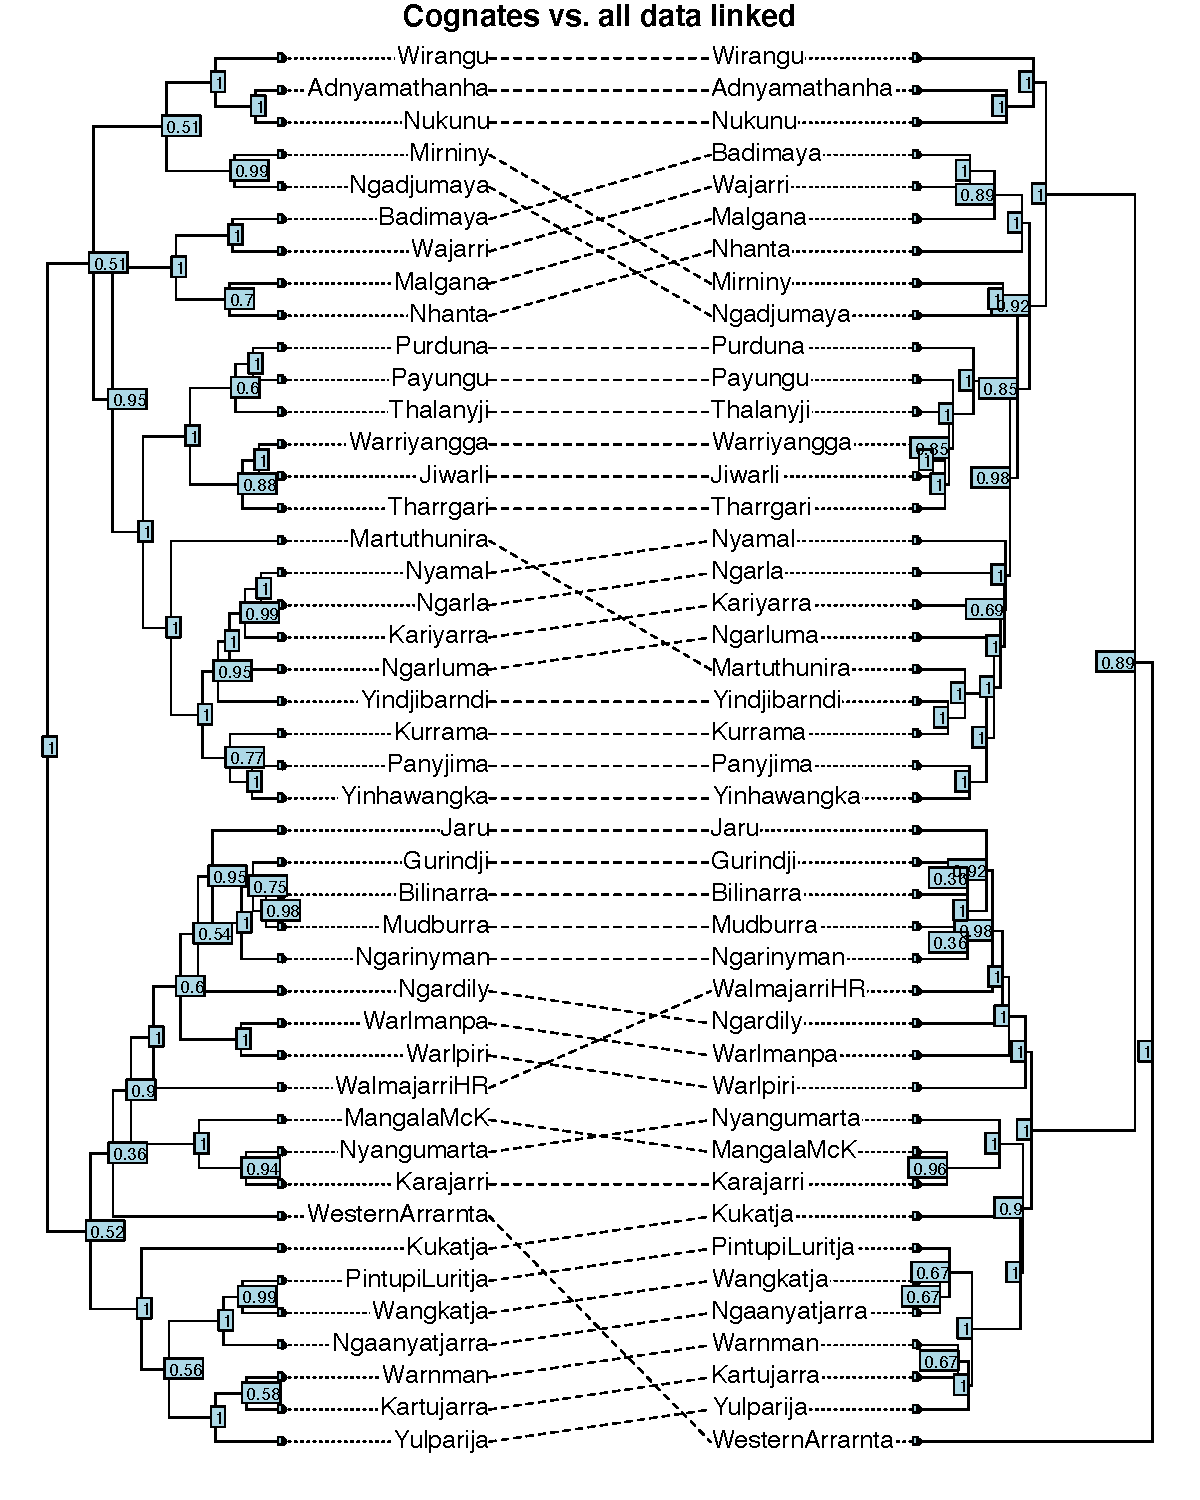
\includegraphics{06-tree-inference/fig/cogs_vs_linked_all.pdf}
\caption[Maximum clade credibility trees for the cognates-only model (from Preliminary Test 2) and the linked model]{\label{fig:cogs-vs-linked-all}Maximum clade credibility trees for the cognates-only model from Preliminary Test 2 (left) and the linked model (right), which was inferred from cognate data and phonotactic data together.}
\end{figure}

The flattening effect of the phonotactic data is evident when MCC trees are calculated for each of the two tree elements of the separate model. Recall that the separate model includes two separate tree elements---one inferred with cognate data only and one inferred with phonotactic data only (both binary and continuous). Maximum clade credibility trees are inferred for each of these elements and plotted in Figure \ref{fig:separate-cogs-vs-phonotactics-all}. Side-by-side, the loss of intermediate tree-like structure is apparent in the phonotactics-only MCC tree. It is perhaps unsurprising then that the linked model, in which a single tree is inferred from all the data together, produces an intermediate level of tree-likeness, less tree-like than the cognates-only model but not as star-like as the phonotactics-only tree in the separate model.

\begin{figure}
\centering
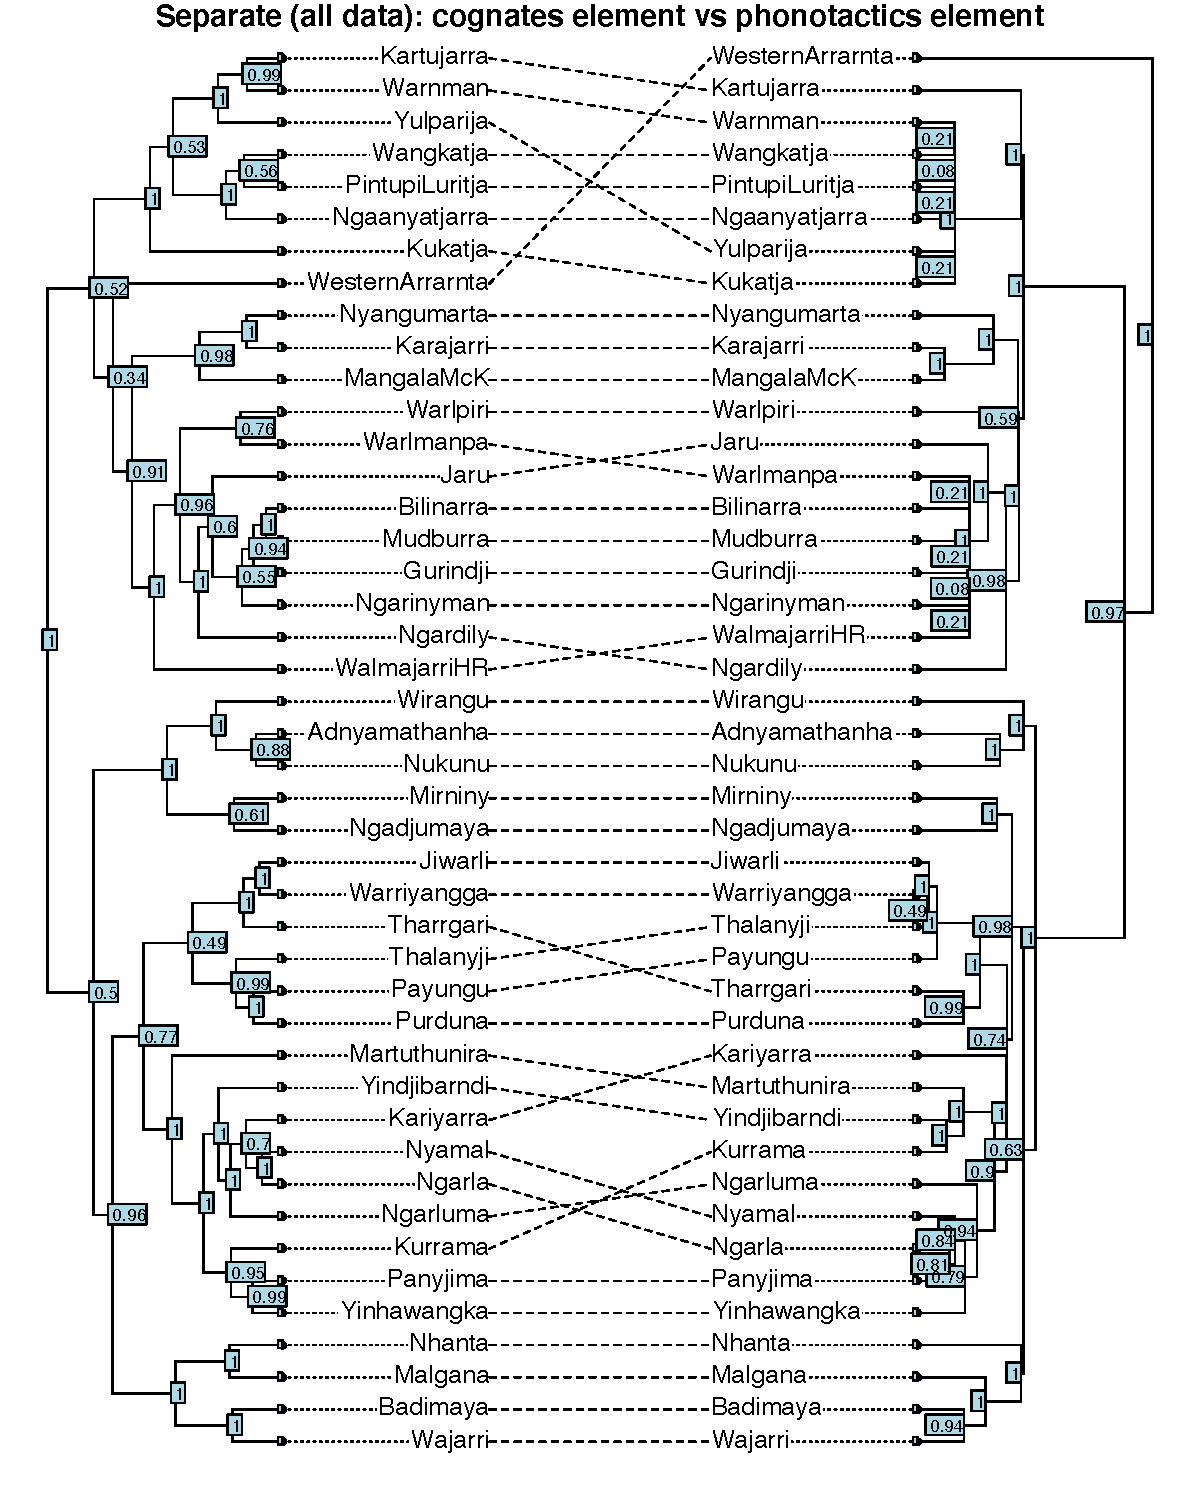
\includegraphics{06-tree-inference/fig/separate_cogs_vs_phonotactics_alldata.pdf}
\caption[Maximum clade credibility trees from the separate model]{\label{fig:separate-cogs-vs-phonotactics-all}Maximum clade credibility trees from the separate model. The tree inferred from cognate data only is depicted on the left, the tree inferred from phonotactics only is on right. The flatter, star-like topology and low clade support values in the tree on the right is suggestive of non-treelike signal in the phonotactics data.}
\end{figure}

\hypertarget{follow-up-test}{%
\section{Follow-up test: Removing binary biphone data}\label{follow-up-test}}

Upon reviewing results of the main test, one initial hypothesis was that the binary biphone data, which we expected would contain a little phylogenetic signal but to a relatively low degree, might be having an outsized influence on likelihood calculations in BEAST. This relatively homogenous dataset, we reasoned, might be driving star-like tree signal in the tree topologies and increasing uncertainty in the analysis. In the likelihood calculations for our models, each data partition is effectively weighted proportionately to the amount of data within it (not due to a particular analytical decision but just because of the way BEAST is presently implemented). Our models contain 1,097 binary lexical cognate characters and 2,236 binary biphone characters, so the cognate data gets outweighed over 2-to-1 despite our prior expectation that the cognate data should be relatively more informative.

To test this hypothesis, we ran one follow-up test which is a replication of the linked model from the main test but with the binary biphone data removed. That is, the phylogeny is inferred from lexical cognate data and continuous phonotactic data only. We ran four independent 100-million-state MCMC chains in BEAST. Unfortunately, the new linked model does not seem to produce more stable or consistent convergences than the original linked model presented above. Of the four MCMC chains, two fail to reach stable convergence while the other two converge to slightly different optima in the state space. We err on the side of the chain in the lower likelihood space, which also has the most stable convergence and highest ESS values (1,269 for joint probability and \textgreater{}200 for all other parameters). We discard 10\% burn-in and calculate an MCC tree for the remaining sample. This is plotted in Figure \ref{fig:linked-all-vs-linked}, side-by-side with the MCC tree for the main linked model above. As can be seen, the linked model produces practically identical tree topologies regardless of whether the binary biphone data is included or not. Some differences in clade support values can be observed, but in some instances these values increase with the removal of binary biphone data while in other instances they decrease. Overall, these differences in clade support values seem not to favour one particular tree over the other.

We conclude that the presence of a large partition of binary biphone data in the main study was not unduly impacting likelihood calculations and the MCMC process. The results are largely replicated whether or not this dataset is included in the study.

\begin{figure}
\centering
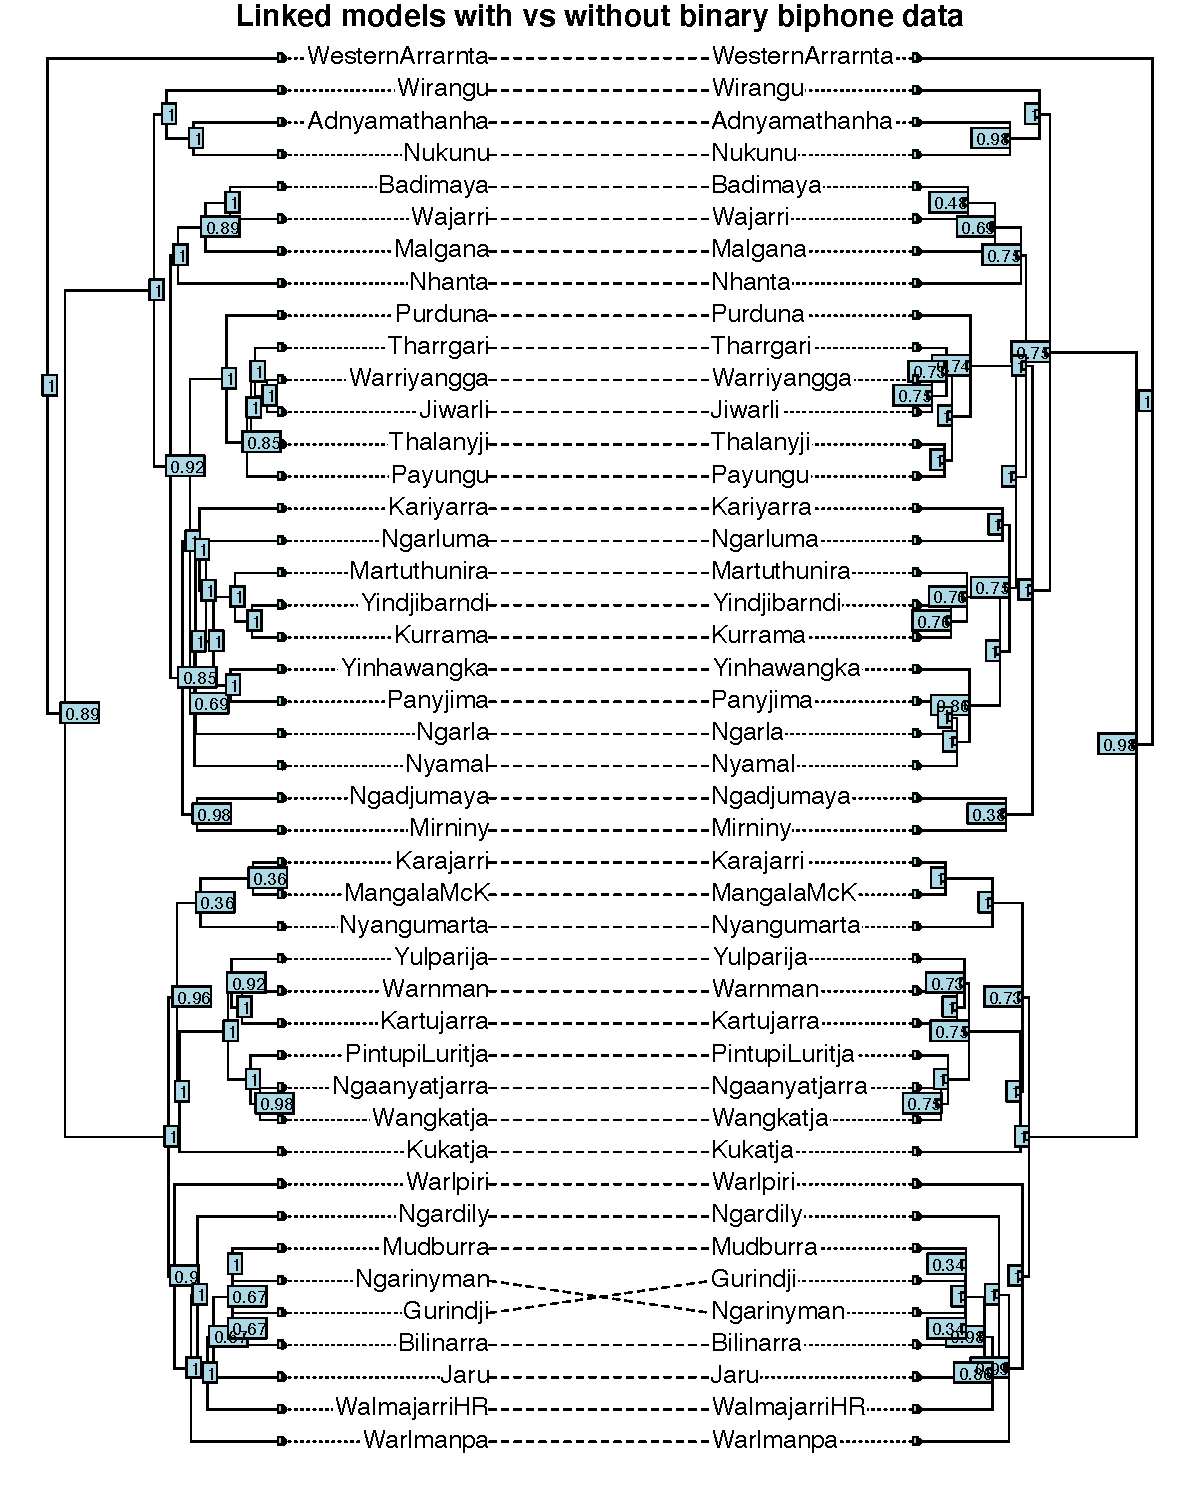
\includegraphics{06-tree-inference/fig/linked_all_vs_linked.pdf}
\caption[Maximum clade credibility trees from the linked model in the Main Test and a follow-up model]{\label{fig:linked-all-vs-linked}Comparison of maximum clade credibility trees from the linked model in the Main Test (left) and a follow-up model which includes cognate data and sound class frequency data, but excludes the binary biphone data. Both trees appear highly congruent, suggesting the binary biphone data had relaively little effect on the results of the Main Test.}
\end{figure}

\hypertarget{pn-tree-discussion}{%
\section{Discussion}\label{pn-tree-discussion}}

In this study, we sought to test the question of whether phonotactic data could help strengthen the inference of phylogenetic signal, when included in a Bayesian computational phylogenetic model in conjunction with more traditional, lexical cognate data. We were motivated by earlier findings that phonotactic data, represented here by binary characters coding the presence or absence of biphones and continuous characters coding the frequency of natural sound classes being followed by other sound classes in biphone sequences, contain phylogenetic signal \autocite{macklin-cordes_phylogenetic_2021}. Our method of testing this hypothesis was to develop two phylogenetic models, a `linked' model and a `separate' model, and infer phylogenies for each using a Bayesian MCMC process implemented in BEAST. In the linked model, tree likelihoods are calculated at each step using existing lexical cognate data from \textcite{bouckaert_origin_2018} and both binary and continuous phonotactic data. In the separate model, two tree likelihoods are calculated, one using cognate data and the other using phonotactic data separately. Marginal likelihoods are estimated to give an indication of overall support for each model. Maximum clade credibility trees are calculated to compare tree topologies and support for particular subclades.

Our results do not support the hypothesis that a better supported phylogeny could be inferred with phonotactic data. To the contrary, we found that the addition of phonotactic data contributed instability and uncertainty into the MCMC process. We also found the MLE process to be unreliable, with extreme divergences between even chains that seemed to reach stable convergence in the same probability space. Inspecting the maximum clade credibility trees, the linked phylogeny seemed to produce an MCC tree broadly comparable to the equivalent phylogeny produced from cognate data only. However, the internal structure of some subgroups did get altered, the posterior clade support values did not, on the whole, improve, and there seemed to be a degree of star-like flattening of the tree shape. To the extent that the linked model recovered the topology of the cognates-only phylogeny, it might be said that it did so in spite of apparent star-like signal in the phonotactic data, rather than with the assistance of phonotactic data. The conclusion is that phonotactic data, in the form presented here, does not strengthen phylogenetic tree inference, at least within the present statistical and computational implementation.

The next question is to what extent these findings represent a genuine negative result, i.e.~evidence for a more general conclusion that phonotactic data does not strengthen phylogenetic tree inference. If this is the case, then future linguistic phylogenetics research should abandon phonotactics as a potential data source. The alternative, however, is that the negative result is attributable to any combination of issues with data acquisition and/or experimental design. In this case, we cannot say the study supports any particular insight into the phylogenetic dynamics of phonotactic systems in human language. Rather, we would require further study, hopefully benefiting from the lessons of the present attempt, before making any conclusions either way. There are reasons, as discussed in the paragraphs that follow, to suspect that this study is an instance of the latter. If that is correct, then the current experiment is best interpreted not as evidence against any particular hypothesis, but rather as evidence for the need for further refinement along the lines we discuss below.

The following points of discussion fall under two main umbrellas. We start with more technical issues relating to experimental design and implementation, then follow with more general, theoretical matters. Firstly, we must consider the difficulties we observed achieving stable, consistent convergences between MCMC chains. It is possible that the development of relatively simple technical fixes might help rectify this issue to some degree. Although 100 million states seems to be enough to reach normal, stable convergence for many chains in this study, others fail to converge or, in some instances, get stuck for a while before managing to escape a local optimum and converging somewhere else very late in the chain. The most obvious solution to this is to try running much longer chains. The difficulty here is operating within computational constraints, as continuous characters increase the running time of the MCMC process by orders of magnitude. The issue of computational feasibility is compounded again as the size of the phylogeny increases. It would be challenging, for example, to run even our present 100 million state chains if we extended our model to the 112-language Pama-Nyungan sample we used in Section \ref{prelim-1}. One second technical fix would be to adjust the operators in BEAST that govern how parameter values shift from state to state. Allowing larger jumps in the parameter space could help the MCMC chain to escape local optima.

A more complex technical issue is the implementation of an evolutionary model for continuous characters. When working with binary datasets in phylogenetic software, one would usually work with a single data partition containing all binary characters or a small number of data partitions. The problem with continuous characters is that the computational time and memory demands of a continuous data partition expand exponentially as the number of continuous characters increases. For example, the sound class biphone dataset that we use in this study would take several years rather than several days to run on identical computing hardware, if implemented as a single data partition. To get around this, we created an individual data partition for each individual character. This brought the study into the realm of reality from a practical standpoint, but at the cost of hugely increasing the number of parameters that form part of the model, because individual rates of evolution and likelihood scores had to be inferred for every character. Besides the question of whether treating each character as its own element in the model is realistic (which we address more below), having such a great array of parameters to estimate likely contributes to uncertainty in the analysis. Future study should consider some option in between the extremes of a single data partition and individual data partitions for all continuous characters. The question is how continuous characters should be partitioned and on what basis. One option is to pre-define data partitions on some linguistically meaningful basis (for example, perhaps grouping characters by the sound class of the first biphone segment). The other option is to infer how the data should be partitioned as part of the analysis. There is work in this space using phylogenetic factor analysis, under active development \autocites{tolkoff_phylogenetic_2018}{hassler_inferring_2020}, and this could be explored in the context of large linguistic datasets of continuous variables in future work. Addressing this issue will have the added benefit of addressing the lack of independence issue.

There are other limitations to the evolutionary model for continuous characters that we used. For one, we use a simple Brownian motion model which allows characters to wander up or down with equal probability. This model has the advantages of being straightforward to implement with existing software and also aligns with earlier work by \textcite{macklin-cordes_phylogenetic_2021}. But it also fails to fully encapsulate the way that biphone frequencies are likely to change over time. One question to consider is what a more realistic model of evolution would look like for frequency-based phonotactic characters. To answer this, we need to think about the causal forces of language change that shape these frequencies. We note two such forces here. The first is the introduction of new vocabulary to a language via lexical innovation or borrowing. Each new word entering a lexicon will alter minutely the frequencies of biphone transitions in the language (similarly, transition frequencies will decline as words are replaced or fall out of usage). This is the kind of gradual accumulation of changes that we might expect to follow a Brownian motion-like pattern of evolution (although maybe the rates of going up and down are not equal). Further, since speakers show a preference for high frequency phonotactic sequences over low frequency sequences when coining new words, we might expect this accumulation of changes to follow some a kind of `rich-get-richer' preferential attachment process which would result in the kind of skewed frequency distributions that we observe. Also, when languages borrow vocabulary, the trend is for foreign words with disfavoured phonotactic sequences to shift towards more natively preferred patterns (sometimes gradually over a long period of time, e.g.~in some French borrowings in English, stress has shifted to English pattern but not yet in others; see also \textcite{crawford_adaptation_2009} on Japanese), which would strengthen this kind of preferential attachment process and also keep phonotactic frequency data historically conservative. The second major force on biphone frequencies is regular sound change. We would expect regular sound changes to result in sudden jumps in the frequencies of affected biphones, sometimes to 0 or 1. For example, if a language includes heterorganic nasal+stop sequences that subsequently undergo place assimilation, this will result in a sudden jump, rather than a gradual drift in frequencies from heterorganic nasal+stop sound class characters to their homorganic counterparts. Our binary characters capture some of these effects to a limited extent. For example, in the place assimilation example above, certain biphones will switch from `1' to `0'. In other instances, sound changes could cause characters to switch from missing all together to some non-missing value or vice versa. For example, if a contrastive vowel length distinction emerges, certain biphones (those with long vowels) will go from being a gap to `1' in the binary biphone data for that language. In the case of a merger between short and long vowels, the opposite will be true. Our model, at present, does not obviously account well for regular sound change. One option for addressing this in future work may be to include a Lévy process in the model, which allows for gradual drift punctuated by sudden jumps \autocite{uyeda_rethinking_2018}. One final limitation to note is that the frequency data and evolutionary model in this study do not account for measurement error. Wordlists are necessarily a limited representation of the complete, true lexicon of a language, and so particularly in the case of shorter wordlists, there may be a margin of error between the true frequencies in the language and the frequencies we extract from its wordlist. There is evidence to suggest that accounting for measurement error could help improve results \autocite{round_clouded_2019}. Overall, future work will need to consider more carefully how a realistic evolutionary model for continuous characters should be designed and, if necessary, do the heavy lifting of implementing the model in phylogenetic software rather than relying on currently available implementations. Furthermore, more careful re-evaluation of the frequency distributions of phonemes in \textcite{macklin-cordes_re-evaluating_2020} should be replicated at the biphone level.

Any statistical model is necessarily an abstraction of reality. The challenge is striking the right balance between a model that is realistic enough to produce realistic outcomes and abstract enough to be both practical and generalisable. In this study, we may have compromised on the realism of the model too much in order to keep the project computationally feasible with presently available software and hardware. Technological advances in central and graphical processing units and increased computational parallelisation \autocite[e.g.][]{holbrook_massive_2020} will mitigate this dilemma somewhat in future, but additional work will be required to create evolutionary models that are more faithful to the real-world diachronic processes that generate phonotactic frequencies.

A final point is that future research might consider whether phonotactic data has a role in phylogenetic tree inference or some other aspect of linguistic phylogenetics beyond tree inference itself. In biology, there is ongoing debate on whether morphological data is best suited to a ``simultaneous'' approach, where the tree is inferred jointly from morphological and genomic data, versus a ``scaffolding'' approach, where the tree is inferred from genomic data only, then morphological data is used to investigate other phylogenetic questions (e.g.~dating branching events using morphological data from the fossil record) while being constrained to the genomic tree's topology \autocites{de_queiroz_including_1996}{lee_morphological_2015}. We do not take up the topic further here, but an analogous discussion could be had in linguistics. It may be the case that phonotactic data or some other kinds of linguistic data are better suited to a scaffolding-type approach, playing a role in phylogenetic investigations but only through application to a phylogenetic tree topology that has already been inferred using cognate data.

\hypertarget{pn-tree-conclusion}{%
\section{Conclusion}\label{pn-tree-conclusion}}

Following earlier findings that phonotactic data contains phylogenetic signal, we sought to create and evaluate evolutionary models for two basic representations of phonotactic information for a sample of 112 Pama-Nyungan languages---binary biphone data coding the presence or absence of biphones in a lexical wordlist, and sound class biphone frequency data coding the frequencies of forward transitions between sound classes in a lexical wordlist. Subsequently, we attempted to infer a phylogeny of a subset of 44 Pama-Nyungan languages representing the western branch of the family, using phonotactic data in combination with existing lexical cognate data. Although marginal likelihood estimates on their face seem to support a linked model where the phylogeny is inferred jointly from phonotactic and cognate data, over a separate model where separate trees are inferred from phonotactic and cognate data separately, we find that the calculation of these figures is unreliable in this instance. Further, through comparison of maximum clade credibility trees for the linked model versus a cognates-only model, we find that the addition of phonotactic data does not seem to strengthen posterior clade support values. To the contrary, the phonotactic data seems to introduce a modest star-like signal to the phylogeny, leading to a slightly flatter tree structure.

These results, we argue, are likely the result of oversimplifying the model of continuous phonotactic character evolution and introducing too many free parameters to the model in an effort to achieve computational feasibility and operate within the bounds of existing phylogenetic software. Future research should develop the phonotactic evolutionary model further before re-evaluating its place in the task of phylogenetic tree inference. The first step of this process would be to evaluate empirically the frequency distributions of biphone characters and attempt to link them to causal processes (e.g.~mergers and splits of phonemic categories). Secondly, the Brownian motion model of character evolution would be replaced with a model that incorporates the identified frequency distribution from the previous step and allows character values to move in ways consistent with the causal processes. Thirdly, dependencies and correlated evolution between characters would be identified and the dataset partitioned accordingly. Fourthly, matters of the technical implementation and MCMC convergence process would be addressed, perhaps with advances in GPU parallelisation, with the aim of inferring reliable marginal likelihood estimates.

As linguistic phylogeneticists look beyond the cognate for sources of novel insight, we advocate a methodical progression and thorough methodological evaluation, from language change processes to large-scale linguistic evolution.

% ***************************************************
